\documentclass{article}
\usepackage{ctex} % 专为中文排版优化
\usepackage{geometry}
\usepackage{hyperref}
\usepackage{xcolor}
\usepackage{multirow}
\usepackage{array}
\usepackage[table]{xcolor}
\usepackage{graphicx}
\usepackage{amsmath} % 数学公式

\geometry{a4paper, margin=1in}


\title{\textbf{Bomblab实验报告}}
\author{
    \normalsize 唐培严 \\
    \normalsize 2024201638
}
\date{\today}

\begin{document}
\maketitle
\begin{table}[ht]
\centering
\begin{tabular}{|c|c|c|c|c|c|c|c|}
\hline
\rowcolor{gray!20}
总分 & phase 1 & phase\_2 & phase 3 & phase 4 & phase 5 & phase 6 & secret phase \\
\hline
7 & 1 & 1 & 1 & 1 & 1 & 1 & 1 \\
\hline
\end{tabular}
\end{table}
scoreboard截图：
\begin{figure}[ht]
        \centering
        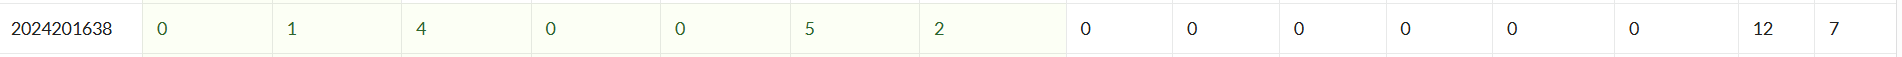
\includegraphics[width=1\linewidth]{1.png}
    \end{figure}

\section{解题报告}
\subsection{phase\_1}
\begin{verbatim}
    Saiverd loclken a wethd, lafz fomdra Lay, Iliffzidra.
\end{verbatim}
\textbf{解题思路：}
\begin{verbatim}
   0x0000555555555439 <+4>:     lea    0x1d40(%rip),%rsi        # 0x555555557180
   0x0000555555555440 <+11>:    call   0x555555555cc7 <strings_not_equal>
   0x0000555555555445 <+16>:    test   %eax,%eax
\end{verbatim}
寄存器\%rsi是第二个参数用的，而第一个参数也就是我们输入的字符就被放到寄存器\%rdi中了。调用string\_not\_equal函数来比较这两个参数，不难知道\%rsi存放的就是这关需要输入的字符串。在gdb中输入“x/s 0x555555557180”查看字符串即可。

\subsection{phase\_2}
\begin{verbatim}
    369469  607463  446925  496795
\end{verbatim}
\textbf{解题思路：}
\begin{verbatim}
   0x000055555555550e <+185>:   add    $0x4,%rbx
   0x0000555555555512 <+189>:   cmp    $0x10,%rbx
   0x0000555555555516 <+193>:   je     0x555555555528 <phase_2+211>
   0x0000555555555518 <+195>:   mov    0x0(%rbp,%rbx,1),%eax
   0x000055555555551c <+199>:   cmp    %eax,(%rsp,%rbx,1)
\end{verbatim}
这道题看似是要计算矩阵相乘的结果，但实际可以通过更取巧的方法得到答案。在反汇编代码这个地方可以看到，程序在依次取我输入的值与(\%rsp,\%rbx,1)比较大小，\%rbx=0x10=16就跳转离开，所以计算得到的结果都被存入(\%rsp,\%rbx,1)这个地方。故只需在0x000055555555551c设置断点，让程序运行到这里，然后“x/4d \$rsp”就可以打印出4个整数值，就是需要我输入的四个整数了。

\subsection{phase\_3}
\begin{verbatim}
    3 D 830
\end{verbatim}
\textbf{解题思路：}
\begin{verbatim}
   0x0000555555555582 <+62>:    cmpl   $0x7,0x10(%rsp)
   0x0000555555555587 <+67>:    ja     0x555555555692 <phase_3+334>
\end{verbatim}
这道题有关跳转表，这里要输入两个整数和一个字符，要求第一个输入的整数不能大于7，故先在solution.txt中随便输入了3，然后跳转到字符比较，如下。
\begin{verbatim}
   0x000055555555560e <+202>:   mov    $0x64,%eax
   0x0000555555555613 <+207>:   cmpl   $0x33e,0x14(%rsp)
   0x000055555555561b <+215>:   je     0x55555555569c <phase_3+344>
   0x000055555555561d <+217>:   call   0x555555555f2c <explode_bomb>
\end{verbatim}
需要输入的字符对应ASCII的0x64即‘d’，再比较下一个整数是否等于0x33e即830。但需要额外注意的是，在“0x000055555555557e <+58>:    xor    \%al,0xf(\%rsp)”这里进行了字符的大小写切换。故输入应是字符‘D’。

\subsection{phase\_4}
\begin{verbatim}
    31 AC
\end{verbatim}
\textbf{解题思路：}
\begin{verbatim}
    0x00005555555557bc <+58>:    cmp    %eax,0xc(%rsp)
\end{verbatim}
这题需要输入一个整数和长度为2的字符串。由这条反汇编代码可以看出，它在进行第一个整数的比较。故设置此处的断点，运行到此处并在gdb中输入“x/d \$rsp + 0xc”即可查看第一个整数需要输入的值。
\begin{verbatim}
   0x00005555555557f8 <+118>:   lea    0x10(%rsp),%rdi
   0x00005555555557fd <+123>:   mov    %rbx,%rsi
   0x0000555555555800 <+126>:   call   0x555555555cc7 <strings_not_equal>
\end{verbatim}
这里进行的是第二个字符串的比较，\%rdi加载的是我输入的字符串，而系统将它和第二个参数存放的寄存器\%rsi比较。故可以知道正确的字符串在\%rsi中，设置断点在0x00005555555557fd处，然后在gdb中输入“x/s \$rsi”即可知道需要输入的字符串。

\subsection{phase\_5}
\begin{verbatim}
    AAAAAI
\end{verbatim}
\textbf{解题思路：}
\begin{verbatim}
   0x0000555555555849 <+9>:     cmp    $0x6,%eax
   0x000055555555584c <+12>:    jne    0x55555555587a <phase_5+58>
   0x000055555555584e <+14>:    mov    %rbx,%rax
   0x0000555555555851 <+17>:    lea    0x6(%rbx),%rdi
   0x0000555555555855 <+21>:    mov    $0x0,%ecx
   0x000055555555585a <+26>:    lea    0x19df(%rip),%rsi   # 0x555555557240 <array.0>
   0x0000555555555861 <+33>:    movzbl (%rax),%edx
   0x0000555555555864 <+36>:    and    $0xf,%edx
   0x0000555555555867 <+39>:    add    (%rsi,%rdx,4),%ecx
\end{verbatim}
这道题要求输入6个字符，然后依次取最后一个字节映射到0~15中，接着按索引取\%rsi寄存器中的元素累加，最后要求总和为0x39即57。不难知道\%rsi中存储了16个整数，因此在gdb中输入“x/16d 0x555555557240”可以得到数组如下：
\begin{verbatim}
   0x555555557240 <array.0>:       2       10      6       1
   0x555555557250 <array.0+16>:    12      16      9       3
   0x555555557260 <array.0+32>:    4       7       14      5
   0x555555557270 <array.0+48>:    11      8       15      13
\end{verbatim}
将57拆成$5\times10+7$，则需要让索引为1和9，对应数组10和7的位置。查询ASCII表可以得到多种答案，我选择的是AAAAAI。

\subsection{phase\_6}
\begin{verbatim}
    1 5 4 3 2 6
\end{verbatim}
\textbf{解题思路：}
\begin{verbatim}
   0x00005555555558fc <+116>:   mov    $0x0,%esi
   0x0000555555555901 <+121>:   mov    (%rsp,%rsi,4),%ecx
   0x0000555555555904 <+124>:   mov    $0x1,%eax
   0x0000555555555909 <+129>:   lea    0x4910(%rip),%rdx     # 0x55555555a220 <node1>
\end{verbatim}
这题要求输出6个数字，不难看出这里是链表的6个节点，在依次取出输入的六个数字对应的节点。
\begin{verbatim}
   0x55555555596e <+230>:   mov    $0x5,%ebp
   0x555555555970 <+232>:   mov    0x8(%rbx),%rbx
   0x555555555974 <+236>:   sub    $0x1,%ebp
   0x555555555977 <+239>:   je     0x55555555598a <phase_6+258>

   0x555555555979 <+241>:   mov    0x8(%rbx),%rax
   0x55555555597d <+245>:   mov    (%rax),%eax
   0x55555555597f <+247>:   cmp    %eax,(%rbx)
   0x555555555981 <+249>:   jle    0x555555555970 <phase_6+232>
\end{verbatim}
从这里可以看到经过5次循环，比较当前节点和下一个节点的值，如果当前节点大于下一个节点的值就会爆炸，故要求升序排列。
\begin{verbatim}
   0x55555555a220 <node1>: 0x00000103      0x00000001      0x5555a230      0x00005555
   0x55555555a230 <node2>: 0x000002cc      0x00000002      0x5555a240      0x00005555
   0x55555555a240 <node3>: 0x0000022b      0x00000003      0x5555a250      0x00005555
   0x55555555a250 <node4>: 0x00000200      0x00000004      0x5555a260      0x00005555
   0x55555555a260 <node5>: 0x00000199      0x00000005      0x5555a170      0x00005555
   0x55555555a170 <node6>: 0x000003b1      0x00000006      0x00000000      0x00000000
\end{verbatim}
故在gdb中输入“x/24x 0x55555555a220”，打印出了前5个节点的信息，但没有第6个节点的信息，仔细观察可以发现，第一个数应该对应的是该节点的值，第二个是索引，第三个和第四个连在一起就是下一个节点对应的地址。故把第5个节点储存的下一个节点的信息拼凑，在gdb中输出“x/4x 0x000055555555a170”，即可得到上述所有节点的信息了。题目要求升序排列，因此顺序为“1 5 4 3 2 6”。

\subsection{secret\_phase}
\begin{verbatim}
    33022
\end{verbatim}
\textbf{解题思路：}进入secret\_phase之前，我跟踪phase\_6的汇编代码进入了phase\_defused函数，进一步跟进发现并没有直接到达secret\_phase函数，于是我“disas phase\_defused”发现有一处字符串判断，只有输入“cipher”之后才会进入secre\_phase。而secret\_phase的反汇编代码并没有给出太多信息，但是它调用了func7函数来做判断处理，故可以推断func7函数的反汇编代码十分关键。在func7中导入了四个数组，分别如下：
\begin{verbatim}
   table1[8] = {-2, -1, 1, 2, 2, 1, -1, -2};
   table2[8] = {1, 2, 2, 1, -1, -2, -2, -1};
   table3[8] = {-1, 0, 0, 1, 1, 0, 0, -1};
   table4[8] = {0, 1, 1, 0, 0, -1, -1, 0};
\end{verbatim}
又结合这几个地方的反汇编代码来看，要求x,y最后分别为4,7.
\begin{verbatim}
   0x0000555555555aca <+286>:   cmp    $0x4,%esi
   0x0000555555555acd <+289>:   jne    0x555555555b3a <func7+398>
   0x0000555555555acf <+291>:   cmp    $0x7,%edx
   0x0000555555555ad2 <+294>:   jne    0x555555555b3a <func7+398>

   0x0000555555555b7b <+463>:   movslq %edx,%rdx
   0x0000555555555b7e <+466>:   mov    $0x0,%ecx
   0x0000555555555b83 <+471>:   cmpb   $0x1,(%rsi,%rdx,1)
   0x0000555555555b87 <+475>:   je     0x555555555b19 <func7+365>
   
   0x0000555555555ba6 <+506>:   movslq %r11d,%rax
   0x0000555555555ba9 <+509>:   mov    $0x0,%ecx
   0x0000555555555bae <+514>:   cmpb   $0x1,(%rdx,%rax,1)
   0x0000555555555bb2 <+518>:   je     0x555555555b19 <func7+365>
\end{verbatim}
再根据题目打印出的提示，判断这个象棋中的马，要求我从（0,0）移动至（4,7），走的路线满足日字型，同时要满足不能让我的落点处为1，也不能让我马脚落点也是1。得到的地图如下：
\begin{verbatim}
0x55555555a1b0 <row0>:  0       0       1       0       0       1       0       0 
0x55555555a1c0 <row1>:  0       0       0       1       0       0       0       1 
0x55555555a1d0 <row2>:  1       0       1       0       0       1       0       0 
0x55555555a1e0 <row3>:  1       0       0       0       0       0       0       0 
0x55555555a1f0 <row4>:  0       1       0       0       1       0       1       0 
0x55555555a200 <row5>:  1       0       0       1       1       0       0       0 
0x55555555a210 <row6>:  0       0       0       0       0       1       0       1 
0x55555555a210 <row6>:  0       0       0       0       0       1       0       1 
\end{verbatim}
自己用手推算可以得出一条路线：$(0,0)\to(2,1)\to(4,2)\to(2,3)\to(3,5)\to(4,7)$，对应到table[0]和table[1]的索引值即“33022”，输入的字符串与上0x7即为索引，则输入可以就是“33022”。

\section{收获与感悟}
做这个lab最大的感想就是这个lab太难了！其实前面的题目倒没有花太久时间，但是secret\_phase确实花了我一个星期都没做出来。我感觉这个lab更多是培养我的敏感性，从一开始完全不知道要做什么，到后面可以比较快速地判断这个地方是在按索引提取序列、这里是在和答案进行比较、这个地方没有第一个参数的寄存器等等。做下来之后的收获确实非常丰富，从期中考试的时候完全不知道gdb操作命令，到现在还算熟练要怎么操作吧。到secret\_phase之前都不知道可以在explode\_bomb这里设置断点，导致炸弹炸了好几次，后来是在和舍友交流的过程中才得知的小技巧，不然都不知道secret\_phase得炸多少次了。

感觉这个lab还有个让我获益的地方就是克服对汇编的恐惧吧，一开始总是觉得这些语言看着就很头大，但是做到后面发现了一些技巧，就感觉其实也不算太难理解，不过secret\_phase确实花了我很久时间，因为我从来没玩过象棋，也不知道什么马走日、马脚这些概念，后来在舍友的提醒下才意识到，逐渐把题目手推出来。

总的来说，这个lab的设置还是相当有挑战性的，但伴随挑战的也是更多的知识和技巧，未来要是有时间我也想再挑战下nuclear\_bomb进一步加深我对汇编的理解和运用。
\end{document}
